\documentclass{standalone}
\usepackage{tikz}
\usetikzlibrary{patterns, positioning}


\begin{document}
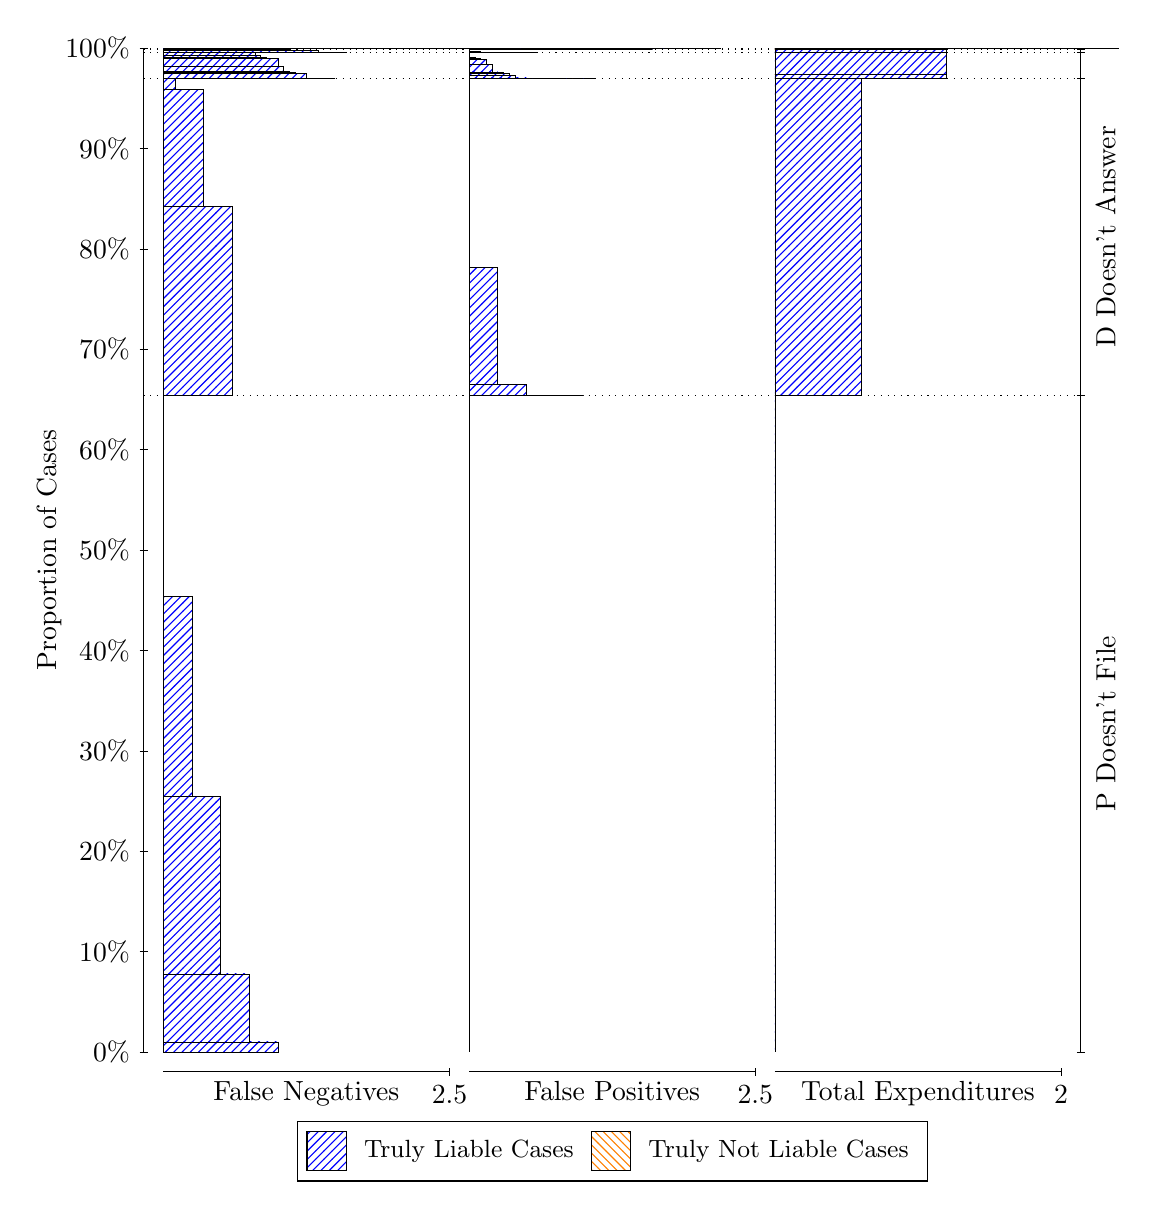
\begin{tikzpicture}
\draw[black, very thin] (1.5,1.75) -- (1.5,14.5);
\node[rotate=90, text=black, anchor=center] at (0.3, 8.125) {Proportion of Cases};
\draw[black, very thin] (1.45,1.75) -- (1.55,1.75);
\node[text=black, anchor=east] at (1.45, 1.75) {0\%};
\draw[black, very thin] (1.45,3.025) -- (1.55,3.025);
\node[text=black, anchor=east] at (1.45, 3.025) {10\%};
\draw[black, very thin] (1.45,4.3) -- (1.55,4.3);
\node[text=black, anchor=east] at (1.45, 4.3) {20\%};
\draw[black, very thin] (1.45,5.575) -- (1.55,5.575);
\node[text=black, anchor=east] at (1.45, 5.575) {30\%};
\draw[black, very thin] (1.45,6.85) -- (1.55,6.85);
\node[text=black, anchor=east] at (1.45, 6.85) {40\%};
\draw[black, very thin] (1.45,8.125) -- (1.55,8.125);
\node[text=black, anchor=east] at (1.45, 8.125) {50\%};
\draw[black, very thin] (1.45,9.4) -- (1.55,9.4);
\node[text=black, anchor=east] at (1.45, 9.4) {60\%};
\draw[black, very thin] (1.45,10.675) -- (1.55,10.675);
\node[text=black, anchor=east] at (1.45, 10.675) {70\%};
\draw[black, very thin] (1.45,11.95) -- (1.55,11.95);
\node[text=black, anchor=east] at (1.45, 11.95) {80\%};
\draw[black, very thin] (1.45,13.225) -- (1.55,13.225);
\node[text=black, anchor=east] at (1.45, 13.225) {90\%};
\draw[black, very thin] (1.45,14.5) -- (1.55,14.5);
\node[text=black, anchor=east] at (1.45, 14.5) {100\%};

\draw[black, very thin] (13.4,1.75) -- (13.4,14.5);
\draw[black, very thin] (13.35,1.75) -- (13.45,1.75);
\node[anchor=west] at (13.35, 1.75) {};
\draw[black, very thin] (13.35,10.09) -- (13.45,10.09);
\node[anchor=west] at (13.35, 10.09) {};
\draw[black, very thin] (13.35,14.114) -- (13.45,14.114);
\node[anchor=west] at (13.35, 14.114) {};
\draw[black, very thin] (13.35,14.448) -- (13.45,14.448);
\node[anchor=west] at (13.35, 14.448) {};
\draw[black, very thin] (13.35,14.485) -- (13.45,14.485);
\node[anchor=west] at (13.35, 14.485) {};
\draw[black, very thin] (13.35,14.492) -- (13.45,14.492);
\node[anchor=west] at (13.35, 14.492) {};
\draw[black, very thin] (13.35,14.5) -- (13.45,14.5);
\node[anchor=west] at (13.35, 14.5) {};

\draw[black, very thin, pattern color=blue, pattern=north east lines] (1.75,1.75) rectangle (3.2033,1.8791);
\draw[black, very thin, pattern color=blue, pattern=north east lines] (1.75,1.8791) rectangle (2.84,2.7414);
\draw[black, very thin, pattern color=blue, pattern=north east lines] (1.75,2.7414) rectangle (2.4767,4.9921);
\draw[black, very thin, pattern color=blue, pattern=north east lines] (1.75,4.9921) rectangle (2.1133,7.5396);
\draw[black, very thin, pattern color=orange, pattern=north west lines] (1.75,7.5396) rectangle (1.75,7.5396);
\draw[black, very thin, pattern color=blue, pattern=north east lines] (1.75,7.5396) rectangle (1.75,10.09);
\draw[black, very thin, pattern color=blue, pattern=north east lines] (1.75,10.09) rectangle (2.622,12.485);
\draw[black, very thin, pattern color=blue, pattern=north east lines] (1.75,12.485) rectangle (2.2587,13.973);
\draw[black, very thin, pattern color=blue, pattern=north east lines] (1.75,13.973) rectangle (1.8953,14.114);
\draw[black, very thin, pattern color=orange, pattern=north west lines] (1.75,14.114) rectangle (1.75,14.114);
\draw[black, very thin, pattern color=blue, pattern=north east lines] (1.75,14.114) rectangle (1.75,14.114);
\draw[black, very thin, pattern color=blue, pattern=north east lines] (1.75,14.114) rectangle (3.93,14.114);
\draw[black, very thin, pattern color=blue, pattern=north east lines] (1.75,14.114) rectangle (3.7847,14.114);
\draw[black, very thin, pattern color=blue, pattern=north east lines] (1.75,14.114) rectangle (3.6393,14.118);
\draw[black, very thin, pattern color=blue, pattern=north east lines] (1.75,14.118) rectangle (3.5667,14.173);
\draw[black, very thin, pattern color=blue, pattern=north east lines] (1.75,14.173) rectangle (3.494,14.178);
\draw[black, very thin, pattern color=blue, pattern=north east lines] (1.75,14.178) rectangle (3.4213,14.19);
\draw[black, very thin, pattern color=blue, pattern=north east lines] (1.75,14.19) rectangle (3.3487,14.204);
\draw[black, very thin, pattern color=blue, pattern=north east lines] (1.75,14.204) rectangle (3.276,14.271);
\draw[black, very thin, pattern color=blue, pattern=north east lines] (1.75,14.271) rectangle (3.2033,14.365);
\draw[black, very thin, pattern color=blue, pattern=north east lines] (1.75,14.365) rectangle (3.1307,14.369);
\draw[black, very thin, pattern color=blue, pattern=north east lines] (1.75,14.369) rectangle (3.058,14.38);
\draw[black, very thin, pattern color=blue, pattern=north east lines] (1.75,14.38) rectangle (2.9853,14.407);
\draw[black, very thin, pattern color=blue, pattern=north east lines] (1.75,14.407) rectangle (2.9127,14.44);
\draw[black, very thin, pattern color=blue, pattern=north east lines] (1.75,14.44) rectangle (2.84,14.442);
\draw[black, very thin, pattern color=blue, pattern=north east lines] (1.75,14.442) rectangle (2.7673,14.442);
\draw[black, very thin, pattern color=blue, pattern=north east lines] (1.75,14.442) rectangle (2.6947,14.442);
\draw[black, very thin, pattern color=blue, pattern=north east lines] (1.75,14.442) rectangle (2.622,14.448);
\draw[black, very thin, pattern color=blue, pattern=north east lines] (1.75,14.448) rectangle (2.5493,14.448);
\draw[black, very thin, pattern color=blue, pattern=north east lines] (1.75,14.448) rectangle (2.4767,14.448);
\draw[black, very thin, pattern color=blue, pattern=north east lines] (1.75,14.448) rectangle (2.404,14.448);
\draw[black, very thin, pattern color=blue, pattern=north east lines] (1.75,14.448) rectangle (2.3313,14.448);
\draw[black, very thin, pattern color=blue, pattern=north east lines] (1.75,14.448) rectangle (2.2587,14.448);
\draw[black, very thin, pattern color=blue, pattern=north east lines] (1.75,14.448) rectangle (2.186,14.448);
\draw[black, very thin, pattern color=blue, pattern=north east lines] (1.75,14.448) rectangle (2.0407,14.448);
\draw[black, very thin, pattern color=blue, pattern=north east lines] (1.75,14.448) rectangle (1.8953,14.448);
\draw[black, very thin, pattern color=orange, pattern=north west lines] (1.75,14.448) rectangle (1.75,14.448);
\draw[black, very thin, pattern color=blue, pattern=north east lines] (1.75,14.448) rectangle (4.0753,14.449);
\draw[black, very thin, pattern color=blue, pattern=north east lines] (1.75,14.449) rectangle (3.712,14.47);
\draw[black, very thin, pattern color=blue, pattern=north east lines] (1.75,14.47) rectangle (3.3487,14.485);
\draw[black, very thin, pattern color=blue, pattern=north east lines] (1.75,14.485) rectangle (2.9853,14.485);
\draw[black, very thin, pattern color=blue, pattern=north east lines] (1.75,14.485) rectangle (2.622,14.485);
\draw[black, very thin, pattern color=orange, pattern=north west lines] (1.75,14.485) rectangle (1.75,14.485);
\draw[black, very thin, pattern color=blue, pattern=north east lines] (1.75,14.485) rectangle (2.622,14.485);
\draw[black, very thin, pattern color=blue, pattern=north east lines] (1.75,14.485) rectangle (2.2587,14.491);
\draw[black, very thin, pattern color=blue, pattern=north east lines] (1.75,14.491) rectangle (1.8953,14.492);
\draw[black, very thin, pattern color=orange, pattern=north west lines] (1.75,14.492) rectangle (1.75,14.492);
\draw[black, very thin, pattern color=blue, pattern=north east lines] (1.75,14.492) rectangle (1.75,14.492);
\draw[black, very thin, pattern color=blue, pattern=north east lines] (1.75,14.492) rectangle (7.5633,14.492);
\draw[black, very thin, pattern color=blue, pattern=north east lines] (1.75,14.492) rectangle (7.2,14.492);
\draw[black, very thin, pattern color=blue, pattern=north east lines] (1.75,14.492) rectangle (6.8367,14.492);
\draw[black, very thin, pattern color=blue, pattern=north east lines] (1.75,14.492) rectangle (6.4733,14.492);
\draw[black, very thin, pattern color=blue, pattern=north east lines] (1.75,14.492) rectangle (6.11,14.492);
\draw[black, very thin, pattern color=blue, pattern=north east lines] (1.75,14.492) rectangle (5.7467,14.492);
\draw[black, very thin, pattern color=blue, pattern=north east lines] (1.75,14.492) rectangle (4.584,14.492);
\draw[black, very thin, pattern color=blue, pattern=north east lines] (1.75,14.492) rectangle (4.2207,14.492);
\draw[black, very thin, pattern color=blue, pattern=north east lines] (1.75,14.492) rectangle (3.8573,14.494);
\draw[black, very thin, pattern color=blue, pattern=north east lines] (1.75,14.494) rectangle (3.494,14.498);
\draw[black, very thin, pattern color=blue, pattern=north east lines] (1.75,14.498) rectangle (3.1307,14.5);
\draw[black, very thin, pattern color=blue, pattern=north east lines] (1.75,14.5) rectangle (2.7673,14.5);
\draw[black, very thin, pattern color=blue, pattern=north east lines] (1.75,14.5) rectangle (2.404,14.5);
\draw[black, very thin, pattern color=blue, pattern=north east lines] (1.75,14.5) rectangle (2.0407,14.5);
\draw[black, very thin, pattern color=orange, pattern=north west lines] (1.75,14.5) rectangle (1.75,14.5);
\draw[black, very thin, pattern color=orange, pattern=north west lines] (5.6333,1.75) rectangle (5.6333,1.75);
\draw[black, very thin, pattern color=blue, pattern=north east lines] (5.6333,1.75) rectangle (5.6333,10.09);
\draw[black, very thin, pattern color=orange, pattern=north west lines] (5.6333,10.09) rectangle (7.0867,10.09);
\draw[black, very thin, pattern color=blue, pattern=north east lines] (5.6333,10.09) rectangle (7.0867,10.09);
\draw[black, very thin, pattern color=blue, pattern=north east lines] (5.6333,10.09) rectangle (6.7233,10.09);
\draw[black, very thin, pattern color=blue, pattern=north east lines] (5.6333,10.09) rectangle (6.36,10.231);
\draw[black, very thin, pattern color=blue, pattern=north east lines] (5.6333,10.231) rectangle (5.9967,11.718);
\draw[black, very thin, pattern color=blue, pattern=north east lines] (5.6333,11.718) rectangle (5.6333,14.114);
\draw[black, very thin, pattern color=orange, pattern=north west lines] (5.6333,14.114) rectangle (7.232,14.114);
\draw[black, very thin, pattern color=blue, pattern=north east lines] (5.6333,14.114) rectangle (7.232,14.114);
\draw[black, very thin, pattern color=orange, pattern=north west lines] (5.6333,14.114) rectangle (7.0867,14.114);
\draw[black, very thin, pattern color=blue, pattern=north east lines] (5.6333,14.114) rectangle (7.0867,14.114);
\draw[black, very thin, pattern color=orange, pattern=north west lines] (5.6333,14.114) rectangle (6.9413,14.114);
\draw[black, very thin, pattern color=blue, pattern=north east lines] (5.6333,14.114) rectangle (6.9413,14.114);
\draw[black, very thin, pattern color=blue, pattern=north east lines] (5.6333,14.114) rectangle (6.8687,14.114);
\draw[black, very thin, pattern color=orange, pattern=north west lines] (5.6333,14.114) rectangle (6.796,14.114);
\draw[black, very thin, pattern color=blue, pattern=north east lines] (5.6333,14.114) rectangle (6.796,14.114);
\draw[black, very thin, pattern color=blue, pattern=north east lines] (5.6333,14.114) rectangle (6.7233,14.114);
\draw[black, very thin, pattern color=orange, pattern=north west lines] (5.6333,14.114) rectangle (6.6507,14.114);
\draw[black, very thin, pattern color=blue, pattern=north east lines] (5.6333,14.114) rectangle (6.6507,14.114);
\draw[black, very thin, pattern color=blue, pattern=north east lines] (5.6333,14.114) rectangle (6.578,14.114);
\draw[black, very thin, pattern color=blue, pattern=north east lines] (5.6333,14.114) rectangle (6.5053,14.119);
\draw[black, very thin, pattern color=blue, pattern=north east lines] (5.6333,14.119) rectangle (6.4327,14.119);
\draw[black, very thin, pattern color=blue, pattern=north east lines] (5.6333,14.119) rectangle (6.36,14.12);
\draw[black, very thin, pattern color=blue, pattern=north east lines] (5.6333,14.12) rectangle (6.2873,14.121);
\draw[black, very thin, pattern color=blue, pattern=north east lines] (5.6333,14.121) rectangle (6.2147,14.155);
\draw[black, very thin, pattern color=blue, pattern=north east lines] (5.6333,14.155) rectangle (6.142,14.182);
\draw[black, very thin, pattern color=blue, pattern=north east lines] (5.6333,14.182) rectangle (6.0693,14.193);
\draw[black, very thin, pattern color=blue, pattern=north east lines] (5.6333,14.193) rectangle (5.9967,14.197);
\draw[black, very thin, pattern color=blue, pattern=north east lines] (5.6333,14.197) rectangle (5.924,14.29);
\draw[black, very thin, pattern color=blue, pattern=north east lines] (5.6333,14.29) rectangle (5.8513,14.357);
\draw[black, very thin, pattern color=blue, pattern=north east lines] (5.6333,14.357) rectangle (5.7787,14.372);
\draw[black, very thin, pattern color=blue, pattern=north east lines] (5.6333,14.372) rectangle (5.706,14.383);
\draw[black, very thin, pattern color=blue, pattern=north east lines] (5.6333,14.383) rectangle (5.6333,14.448);
\draw[black, very thin, pattern color=orange, pattern=north west lines] (5.6333,14.448) rectangle (6.5053,14.448);
\draw[black, very thin, pattern color=blue, pattern=north east lines] (5.6333,14.448) rectangle (6.5053,14.448);
\draw[black, very thin, pattern color=blue, pattern=north east lines] (5.6333,14.448) rectangle (6.142,14.448);
\draw[black, very thin, pattern color=blue, pattern=north east lines] (5.6333,14.448) rectangle (5.7787,14.462);
\draw[black, very thin, pattern color=blue, pattern=north east lines] (5.6333,14.462) rectangle (5.6333,14.485);
\draw[black, very thin, pattern color=orange, pattern=north west lines] (5.6333,14.485) rectangle (7.9587,14.485);
\draw[black, very thin, pattern color=blue, pattern=north east lines] (5.6333,14.485) rectangle (7.9587,14.485);
\draw[black, very thin, pattern color=blue, pattern=north east lines] (5.6333,14.485) rectangle (7.5953,14.485);
\draw[black, very thin, pattern color=blue, pattern=north east lines] (5.6333,14.485) rectangle (7.232,14.486);
\draw[black, very thin, pattern color=blue, pattern=north east lines] (5.6333,14.486) rectangle (6.8687,14.492);
\draw[black, very thin, pattern color=blue, pattern=north east lines] (5.6333,14.492) rectangle (6.5053,14.492);
\draw[black, very thin, pattern color=orange, pattern=north west lines] (5.6333,14.492) rectangle (8.8307,14.492);
\draw[black, very thin, pattern color=blue, pattern=north east lines] (5.6333,14.492) rectangle (8.8307,14.492);
\draw[black, very thin, pattern color=blue, pattern=north east lines] (5.6333,14.492) rectangle (8.4673,14.492);
\draw[black, very thin, pattern color=orange, pattern=north west lines] (5.6333,14.492) rectangle (8.4673,14.492);
\draw[black, very thin, pattern color=blue, pattern=north east lines] (5.6333,14.492) rectangle (8.4673,14.492);
\draw[black, very thin, pattern color=blue, pattern=north east lines] (5.6333,14.492) rectangle (8.104,14.492);
\draw[black, very thin, pattern color=orange, pattern=north west lines] (5.6333,14.492) rectangle (8.104,14.492);
\draw[black, very thin, pattern color=blue, pattern=north east lines] (5.6333,14.492) rectangle (8.104,14.492);
\draw[black, very thin, pattern color=blue, pattern=north east lines] (5.6333,14.492) rectangle (7.7407,14.494);
\draw[black, very thin, pattern color=orange, pattern=north west lines] (5.6333,14.494) rectangle (7.7407,14.494);
\draw[black, very thin, pattern color=blue, pattern=north east lines] (5.6333,14.494) rectangle (7.7407,14.494);
\draw[black, very thin, pattern color=blue, pattern=north east lines] (5.6333,14.494) rectangle (7.3773,14.494);
\draw[black, very thin, pattern color=blue, pattern=north east lines] (5.6333,14.494) rectangle (7.3773,14.498);
\draw[black, very thin, pattern color=blue, pattern=north east lines] (5.6333,14.498) rectangle (7.014,14.5);
\draw[black, very thin, pattern color=blue, pattern=north east lines] (5.6333,14.5) rectangle (6.6507,14.5);
\draw[black, very thin, pattern color=blue, pattern=north east lines] (5.6333,14.5) rectangle (6.2873,14.5);
\draw[black, very thin, pattern color=orange, pattern=north west lines] (5.6333,14.5) rectangle (5.6333,14.5);
\draw[black, very thin, pattern color=blue, pattern=north east lines] (5.6333,14.5) rectangle (5.6333,14.5);
\draw[black, very thin, pattern color=orange, pattern=north west lines] (9.5167,1.75) rectangle (9.5167,1.75);
\draw[black, very thin, pattern color=blue, pattern=north east lines] (9.5167,1.75) rectangle (9.5167,10.09);
\draw[black, very thin, pattern color=orange, pattern=north west lines] (9.5167,10.09) rectangle (10.607,10.09);
\draw[black, very thin, pattern color=blue, pattern=north east lines] (9.5167,10.09) rectangle (10.607,14.114);
\draw[black, very thin, pattern color=orange, pattern=north west lines] (9.5167,14.114) rectangle (11.697,14.114);
\draw[black, very thin, pattern color=blue, pattern=north east lines] (9.5167,14.114) rectangle (11.697,14.161);
\draw[black, very thin, pattern color=orange, pattern=north west lines] (9.5167,14.161) rectangle (11.697,14.161);
\draw[black, very thin, pattern color=blue, pattern=north east lines] (9.5167,14.161) rectangle (11.697,14.448);
\draw[black, very thin, pattern color=orange, pattern=north west lines] (9.5167,14.448) rectangle (11.697,14.448);
\draw[black, very thin, pattern color=blue, pattern=north east lines] (9.5167,14.448) rectangle (11.697,14.485);
\draw[black, very thin, pattern color=orange, pattern=north west lines] (9.5167,14.485) rectangle (11.697,14.485);
\draw[black, very thin, pattern color=blue, pattern=north east lines] (9.5167,14.485) rectangle (11.697,14.492);
\draw[black, very thin, pattern color=orange, pattern=north west lines] (9.5167,14.492) rectangle (13.877,14.492);
\draw[black, very thin, pattern color=blue, pattern=north east lines] (9.5167,14.492) rectangle (13.877,14.494);
\draw[black, very thin, pattern color=orange, pattern=north west lines] (9.5167,14.494) rectangle (13.877,14.494);
\draw[black, very thin, pattern color=blue, pattern=north east lines] (9.5167,14.494) rectangle (13.877,14.5);
\draw[black, dotted] (1.5,10.09) -- (13.4,10.09);
\draw[black, dotted] (1.5,14.114) -- (13.4,14.114);
\draw[black, dotted] (1.5,14.448) -- (13.4,14.448);
\draw[black, dotted] (1.5,14.485) -- (13.4,14.485);
\draw[black, dotted] (1.5,14.492) -- (13.4,14.492);
\draw[black, very thin] (1.75,1.5) -- (5.3833,1.5);
\node[text=black, anchor=north] at (3.5667, 1.5) {False Negatives};
\draw[black, very thin] (5.3833,1.45) -- (5.3833,1.55);
\node[text=black, anchor=north] at (5.3833, 1.45) {2.5};

\draw[black, very thin] (5.6333,1.5) -- (9.2667,1.5);
\node[text=black, anchor=north] at (7.45, 1.5) {False Positives};
\draw[black, very thin] (9.2667,1.45) -- (9.2667,1.55);
\node[text=black, anchor=north] at (9.2667, 1.45) {2.5};

\draw[black, very thin] (9.5167,1.5) -- (13.15,1.5);
\node[text=black, anchor=north] at (11.333, 1.5) {Total Expenditures};
\draw[black, very thin] (13.15,1.45) -- (13.15,1.55);
\node[text=black, anchor=north] at (13.15, 1.45) {2};

\node[text=black, centered, rotate=90] at (13.72, 5.9198) {P Doesn't File};
\node[text=black, centered, rotate=90] at (13.72, 12.102) {D Doesn't Answer};





\draw (7.449999999999999,1.5) node[draw=none] (baseCoordinate) {};
\begin{scope}[align=center]
        \matrix[scale=0.5, draw=black, below=0.5cm of baseCoordinate, nodes={draw}, column sep=0.1cm]{
            \node[rectangle, draw, minimum width=0.5cm, minimum height=0.5cm, pattern color=blue, pattern=north east lines] {}; &
            \node[draw=none, font=\small, text=black] (B) {Truly Liable Cases}; &
            \node[rectangle, draw, minimum width=0.5cm, minimum height=0.5cm, pattern color=orange, pattern=north west lines] {}; &
            \node[draw=none, font=\small, text=black] (B) {Truly Not Liable Cases}; \\
            };
\end{scope}

\end{tikzpicture}
\end{document}